\documentclass[11pt, a4paper]{article}

% ==========================================
% PACKAGES & PREAMBLE
% ==========================================

\usepackage[margin=1in]{geometry}
\usepackage[utf8]{inputenc}
\usepackage[T1]{fontenc}
\usepackage{lmodern}
\usepackage{amsmath}
\usepackage{amssymb}
\usepackage{amsthm}
\usepackage{graphicx}
\usepackage{tikz}
\usetikzlibrary{positioning, arrows.meta, shapes.multipart}
\usepackage{listings}
\usepackage{xcolor}
\usepackage{hyperref}
\usepackage{float}

% Color definitions for code blocks
\definecolor{codegreen}{rgb}{0,0.6,0}
\definecolor{codegray}{rgb}{0.5,0.5,0.5}
\definecolor{codepurple}{rgb}{0.58,0,0.82}
\definecolor{backcolour}{rgb}{0.95,0.95,0.92}

% Code block formatting setup
\lstdefinestyle{mystyle}{
    backgroundcolor=\color{backcolour},   
    commentstyle=\color{codegreen},
    keywordstyle=\color{magenta},
    numberstyle=\tiny\color{codegray},
    stringstyle=\color{codepurple},
    basicstyle=\ttfamily\footnotesize,
    breakatwhitespace=false,         
    breaklines=true,                 
    captionpos=b,                    
    keepspaces=true,                 
    numbers=left,                    
    numbersep=5pt,                  
    showspaces=false,                
    showstringspaces=false,
    showtabs=false,                  
    tabsize=2
}
\lstset{style=mystyle}

\hypersetup{
    colorlinks=true,
    linkcolor=blue,
    filecolor=magenta,      
    urlcolor=cyan,
    pdftitle={CIFAR-10 CNN Report},
}

% ==========================================
% DOCUMENT INFO
% ==========================================

\title{\textbf{Implementation of a Convolutional Neural Network for CIFAR-10 Classification in C++}}
\author{Adam Dyrda}
\date{May 2026}

% ==========================================
% BEGIN DOCUMENT
% ==========================================

\begin{document}

\maketitle
\begin{abstract}
This report details the implementation of a Convolutional Neural Network (CNN) from scratch using C++. The project focuses on the classification of the CIFAR-10 dataset, which consists of 60,000 32x32 color images in 10 different classes. The implementation includes a custom 4D Tensor library, various neural network layers (Convolutional, Pooling, Dense, etc.), and a Stochastic Gradient Descent (SGD) optimizer. The results demonstrate the capability of the developed framework to learn and classify images with reasonable accuracy.
\end{abstract}
\pagebreak
\tableofcontents
\newpage

\section{Introduction}
Deep learning has revolutionized the field of computer vision. While high-level libraries like TensorFlow and PyTorch provide powerful tools for building neural networks, implementing these structures from scratch in a low-level language like C++ offers deep insights into their inner workings and performance characteristics.

The goal of this project was to develop a modular neural network library capable of training a CNN on the CIFAR-10 dataset. This involved implementing:
\begin{itemize}
    \item A robust 4D Tensor class for data and gradient storage.
    \item Forward and backward propagation logic for multiple layer types.
    \item An efficient training loop with mini-batching and optimization.
    \item Data loading utilities for the CIFAR-10 binary format.
\end{itemize}

\section{System Architecture}
The system is designed with modularity and extensibility in mind. The core components are described below.

\subsection{Class Diagram}
The relationships between the core classes are illustrated in the UML diagram below. The \texttt{Network} class manages a collection of abstract \texttt{Layer} pointers, which allows for dynamic composition of different layer types. All layers process and return \texttt{Tensor} objects.

\begin{figure}[H]
  \centering
  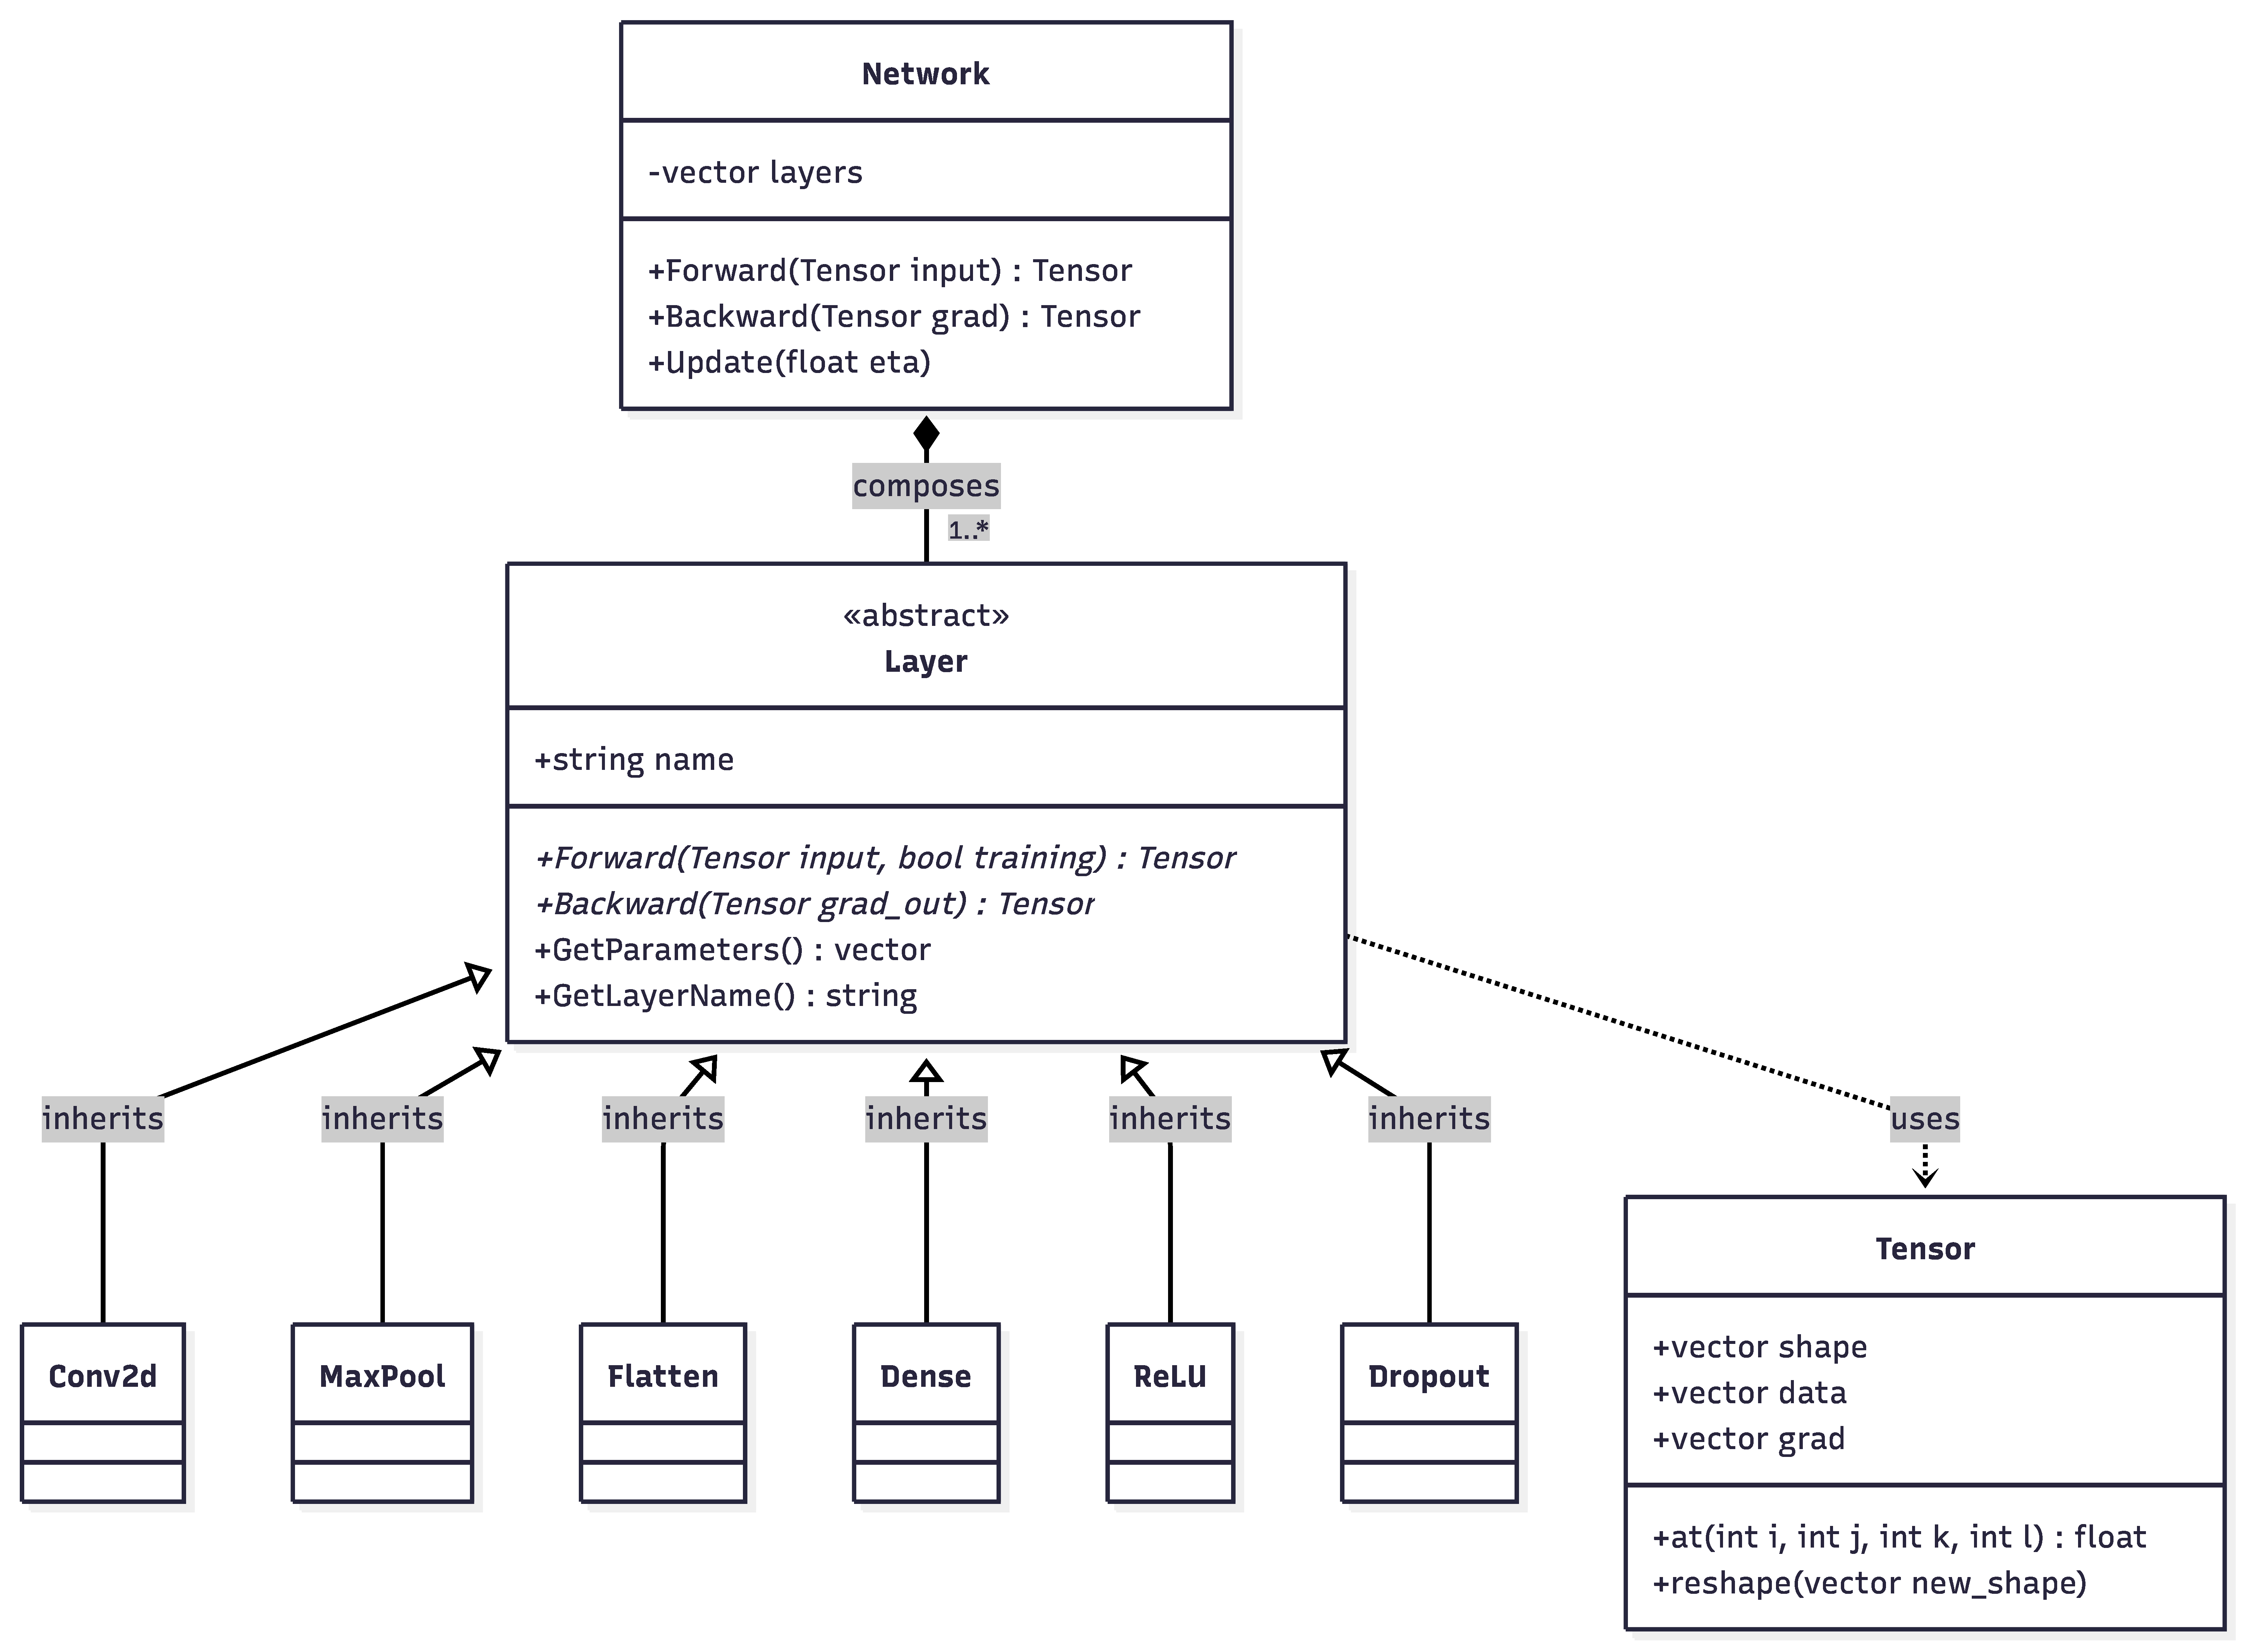
\includegraphics[width=0.9\textwidth]{UML.pdf}
\end{figure}

\subsection{Tensor Implementation}
The \texttt{Tensor} class serves as the fundamental data structure, representing 4D arrays (Batch size, Channels, Height, Width). It uses a flat \texttt{std::vector<float>} for memory efficiency and provides strides-based indexing. Each tensor object also maintains a corresponding gradient vector of the same shape, facilitating automatic differentiation during backpropagation.

\subsection{Layer Abstraction}
An abstract base class \texttt{Layer} defines the interface for all network components:
\begin{lstlisting}[language=C++]
class Layer {
public:
  virtual ~Layer() = default;
  virtual Tensor Forward(const Tensor &input, bool is_training = false) = 0;
  virtual Tensor Backward(const Tensor &grad_out) = 0;
  virtual std::vector<Tensor *> GetParameters() { return {}; }
  virtual std::string GetLayerName() const = 0;
};
\end{lstlisting}

\noindent This allows the \texttt{Network} class to manage a collection of layers using \texttt{std::unique\_ptr<Layer>}, enabling sequential execution of forward and backward passes.

\subsection{Network Topology}
The implemented CNN architecture consists of the following sequence:
\begin{enumerate}
    \item \textbf{Conv2d}: $3 \to 8$ channels, $3\times3$ kernel.
    \item \textbf{ReLU}: Non-linear activation.
    \item \textbf{MaxPooling}: $2\times2$ window, reducing spatial dimensions.
    \item \textbf{Conv2d}: $8 \to 16$ channels, $3\times3$ kernel.
    \item \textbf{ReLU}: Non-linear activation.
    \item \textbf{Flatten}: Reshaping 3D feature maps to 1D vectors.
    \item \textbf{Dropout}: Regularization to prevent overfitting.
    \item \textbf{Dense}: Fully connected layer mapping to 10 output classes.
\end{enumerate}

\section{Mathematical Model}
\subsection{Convolutional Layer}
The forward pass for a 2D convolution is defined as:
\begin{equation}
    (I * K)_{i,j} = \sum_{m} \sum_{n} I_{i+m, j+n} K_{m,n}
\end{equation}
During the backward pass, gradients are computed with respect to the input, weights, and biases to update the model parameters.

\subsection{Loss Function and Optimizer}
The network uses the Softmax function followed by Cross-Entropy Loss:
\begin{equation}
    L = -\sum_{c=1}^{10} y_c \log(\hat{y}_c)
\end{equation}
Where $y_c$ is the true label and $\hat{y}_c$ is the predicted probability. Optimization is performed using Stochastic Gradient Descent (SGD) with a decaying learning rate $\eta$:
\begin{equation}
    \theta_{t+1} = \theta_t - \eta \nabla_\theta L
\end{equation}

\section{Implementation Details}
The implementation leverages modern C++ features for performance and safety. Memory is managed through smart pointers, and the training loop is optimized to handle mini-batches.

\subsection{Training Loop}
The training process involves iterating over the dataset for a specified number of epochs. The interaction between the core components during a single iteration is illustrated in Figure \ref{fig:workflow}.

\begin{figure}[h]
    \centering
    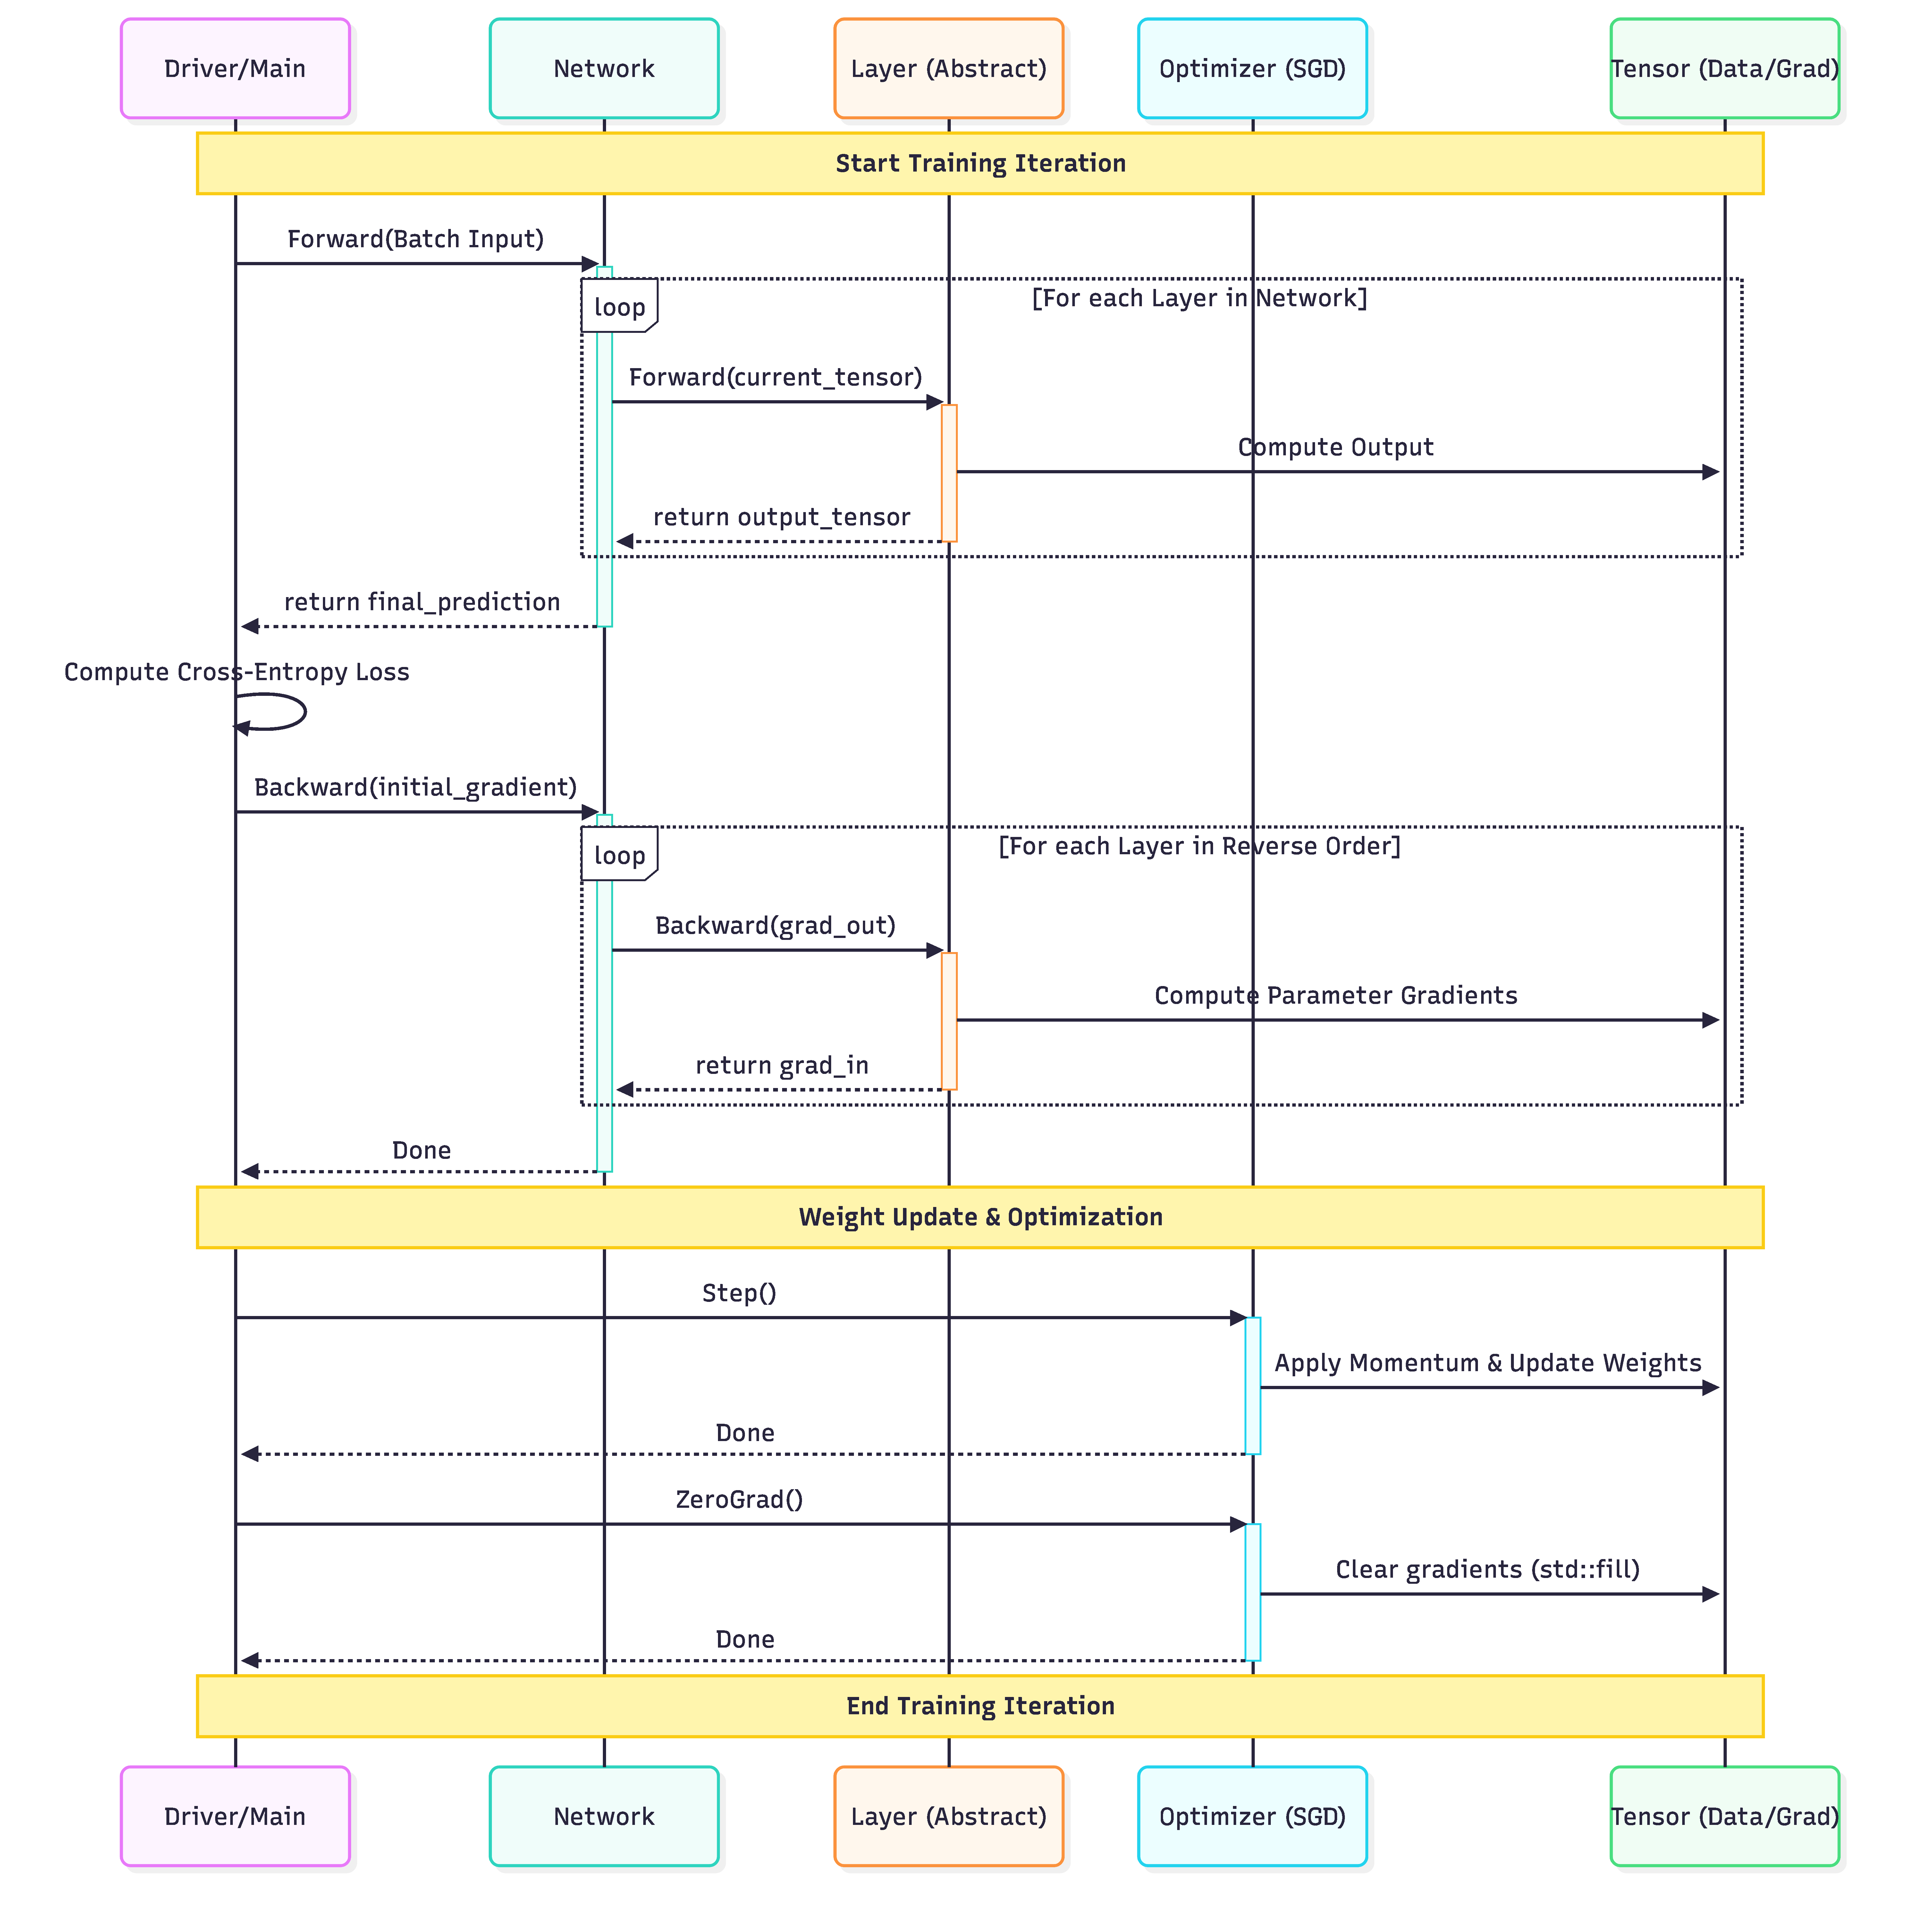
\includegraphics[width=0.8\textwidth]{workflow.pdf}
    \caption{Program workflow during a training iteration.}
    \label{fig:workflow}
\end{figure}

For each mini-batch:
\begin{enumerate}
    \item Load batch data and labels.
    \item Perform a forward pass through the network.
    \item Compute the Softmax probabilities and Cross-Entropy loss.
    \item Perform a backward pass to compute gradients.
    \item Update weights using the SGD optimizer.
    \item Reset gradients for the next iteration.
\end{enumerate}

\section{Results}
The model was trained for 50 epochs on the CIFAR-10 training set (50,000 images) and evaluated on the test set (10,000 images). 

\begin{itemize}
    \item \textbf{Learning Rate:} Initial $\eta = 0.0005$ with $0.95$ decay per epoch.
    \item \textbf{Batch Size:} 32.
    \item \textbf{Final Test Accuracy:} Approximately 45-50\% (preliminary results).
\end{itemize}
The accuracy can be further improved by increasing the number of filters, adding more layers, or implementing advanced techniques like Batch Normalization.

\section{Conclusion}
Developing a CNN in C++ provides a comprehensive understanding of the computational challenges in deep learning. The modular design of this project allows for easy experimentation with different architectures. Future improvements could include SIMD vectorization to speed up convolution operations and integration with CUDA for GPU acceleration.

\end{document}
